\documentclass[9pt,twocolumn,twoside,lineno]{pnas-new}
% Use the lineno option to display guide line numbers if required.

\templatetype{pnasresearcharticle} % Choose template 
% {pnasresearcharticle} = Template for a two-column research article
% {pnasmathematics} %= Template for a one-column mathematics article
% {pnasinvited} %= Template for a PNAS invited submission

\title{Cavity analysis of the brain networks via persistent homology}

% Use letters for affiliations, numbers to show equal authorship (if applicable) and to indicate the corresponding author
\author[a,1]{B. Ülgen Kılıç}

\affil[a]{State University of New York, University at Buffalo, Department of Mathematics}


% Please give the surname of the lead author for the running footer
\leadauthor{Kılıç} 

% Please add here a significance statement to explain the relevance of your work
\significancestatement{Human brain is one of the absolute unknowns of the modern times starting with Ramon y Cajal and Golgi. Recent work has shown that by considering it as a complex system and modeling it as a network, then focusing on the network properties might shed light on this mystery. Toolbox for network analysis is limited and fully exploited already to investigate the architecture of the brain over the past decade. So, network neuroscience is in need of either development of new machinery or employment of already existing machinery from other disciplines. Algebraic topology is a well studied branch of mathematics whose applications have started to gain attention recently by various research areas. Here, we are applying persistent homology to understand the mechanisms driving this most advanced product of the natural selection as well as the origins of consciousness. }

% Please include corresponding author, author contribution and author declaration information
\correspondingauthor{\textsuperscript{1}e-mail: bengieru@buffalo.edu}

% Keywords are not mandatory, but authors are strongly encouraged to provide them. If provided, please include two to five keywords, separated by the pipe symbol, e.g:
\keywords{Structural/Functional Brain Network $|$ Network Neuroscience $|$ Persistent Homology $|$ Homological Scaffolds } 

\begin{abstract}
The network science has proven to be an exceptional tool for modeling and analyzing the real world systems in the past couple of decades. Among all the complex systems, the neural system has it's own unique corner in terms of it's self referencing nature due to the functional complexity of it. There is a caveat here by Godel, a famous mathematician, logician and philosopher, stating that it might not be possible to fully resolve the mysteries of a formal system for an observer inside of the system meaning that we are trying to understand the brain via our brain again. Is brain really that complex that it is able to understand it's own complexity? We don't know the answer yet, since we are far from understanding the all capabilities of the brain at the moment. However, this doesn't mean that we are not going to expand the frontiers as much as we can in neuroscience by utilizing different tools. With this motivation in mind, we want to combine the knowledge from a well-studied branch of mathematics, algebraic topology, and persistent homology in particular is going to be the main tool we are employing. Our aim is to bypass the edges with low weight and focus on relatively strong edges with respect to their surrounding without applying any sort of thresholding. We start by examining the evolution of the clique structures in a structural brain network, resting state functional brain network and task state functional brain network. Then, we will pull out these regions from the networks and aggregate on top of each other to construct homological scaffolds of the brain. 
\end{abstract}

\dates{This manuscript was compiled on \today}
\doi{\url{www.pnas.org/cgi/doi/10.1073/pnas.XXXXXXXXXX}}

\begin{document}

\maketitle
\thispagestyle{firststyle}
\ifthenelse{\boolean{shortarticle}}{\ifthenelse{\boolean{singlecolumn}}{\abscontentformatted}{\abscontent}}{}

% If your first paragraph (i.e. with the \dropcap) contains a list environment (quote, quotation, theorem, definition, enumerate, itemize...), the line after the list may have some extra indentation. If this is the case, add \parshape=0 to the end of the list environment.
\dropcap{I}t has been hypothesized that the human brain network has scale-free topology, meaning that its degree distribution is given by the controversial power law\cite{smallworld1,smallworld2} whereas some others have shown why human brain doesn't have scale-free topology\cite{smallworld3}. Degree of a node in a network is the fundamental network measure determining the topology of the network. Moreover, network analysis so far is based on drawing tools from graph theory to quantify the network properties such as clustering coefficient, modularity and distribution of motif and hub structures which can actually provide meaningful information about the way this complex system works\cite{graphtheory,netwmeasure}. There are several state-of-the-art methods of constructing the brain networks from the various measurements \cite{stateoftheart} which most of the time corresponds to either structure or the function of the mammalian  brain.  In a large scale brain network, nodes are described by brain regions in the cortical and subcortical areas. In a structural brain network, the relations between the nodes are defined by white matter tracts which are obtained by DSI. On the other hand, in a functional brain network, links are given by the magnitudes of functional correlations in activity obtained by fMRI. So, the way we analyze the brain via network science depends completely on the network that we use since the nature of the connections are derived from different choices.


\begin{figure}%[tbhp]
\centering
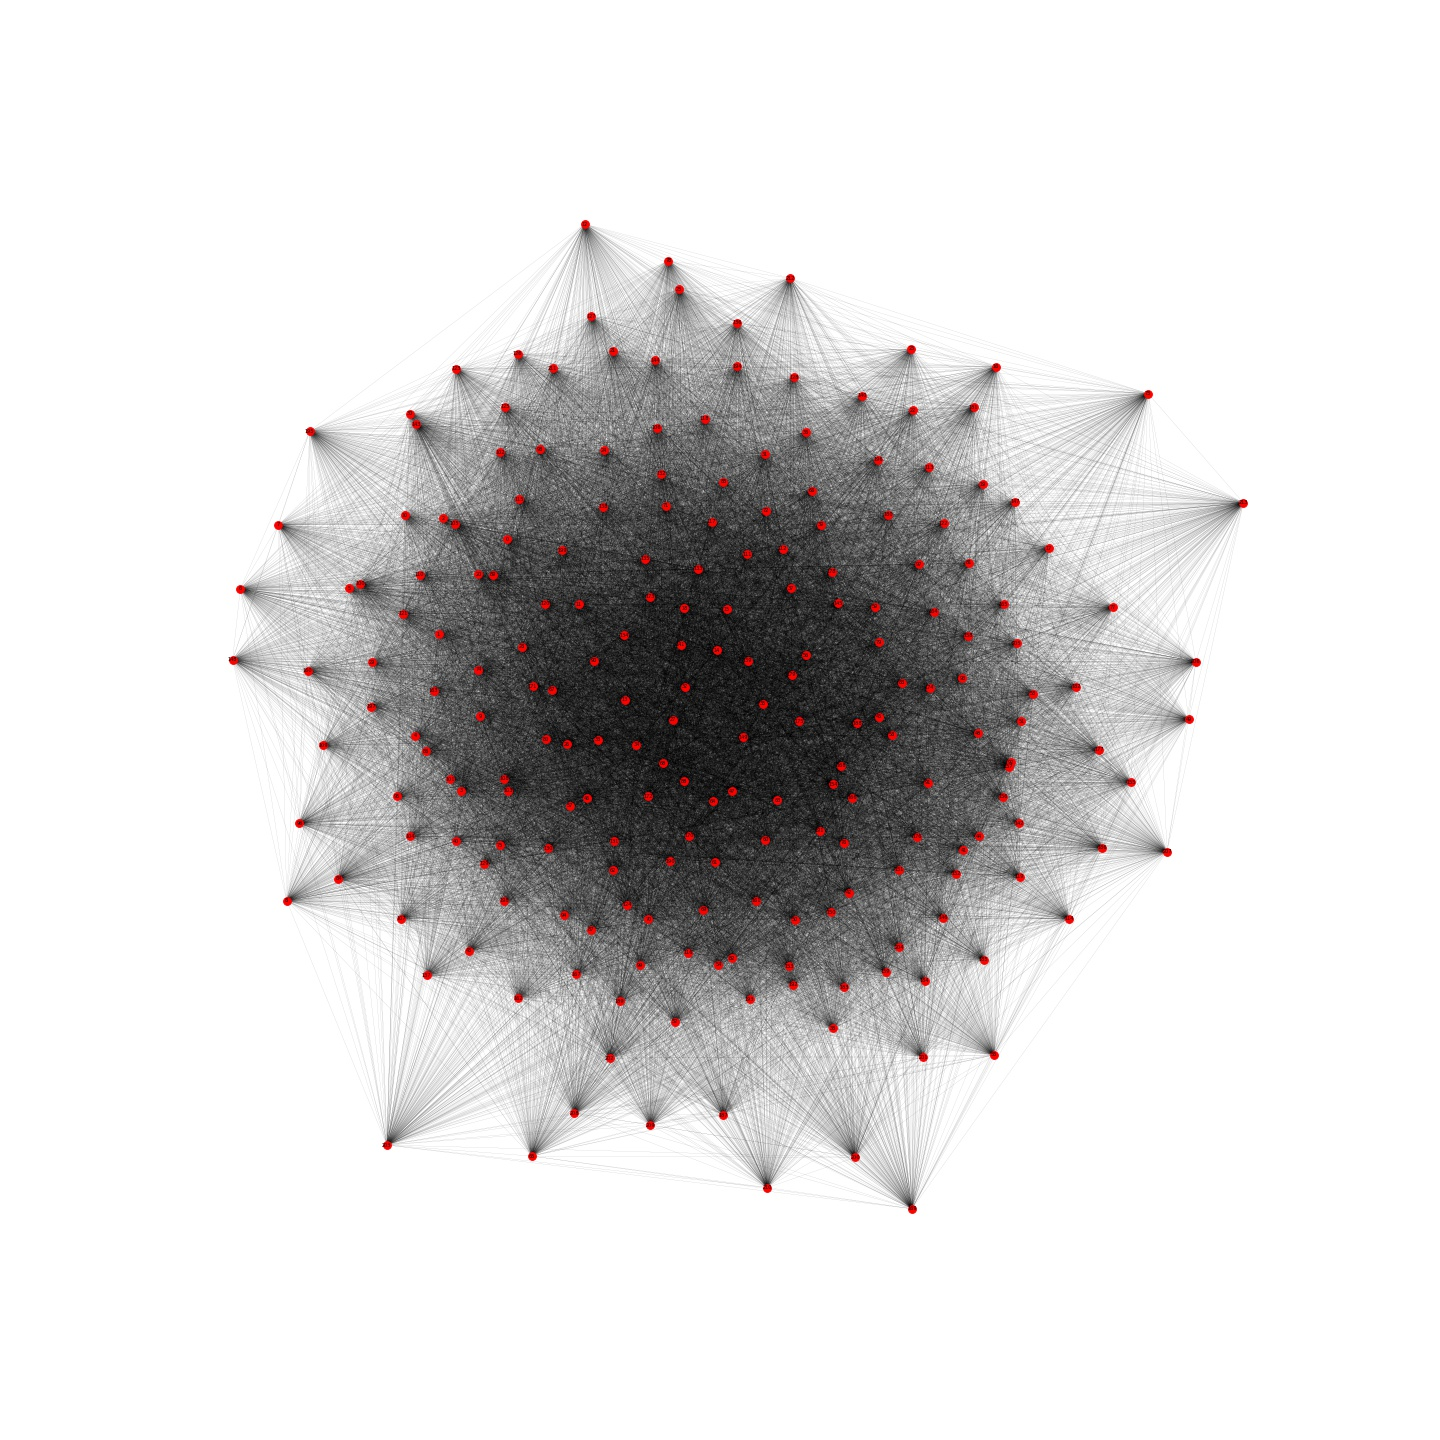
\includegraphics[width=.8\linewidth]{spring.jpg}
\caption{Just to give a taste of the object that we are dealing with: visualization of the functional brain network. Since this is already an overly complicated picture, we don't bother to draw the other two. Each node corresponds to a brain region and edges are defined by functional correlation between  these regions}
\label{fig:network}
\end{figure}

Both the structural and functional network constructions, which generally yield a fully connected and weighted adjacency matrix, from the brain imaging data involve a thresholding of the edge weights leading to lose structural and functional meaning because we do not have a generally accepted criteria for determining a proper threshold. So, instead of trying to come up with a proper threshold for network analysis that may not work for different populations or cognitive conditions, we propose a multiscale framework that models all brain networks generated over every possible threshold and traces the evolution of network changes over different thresholds. This method is going to enable us to capture the information over all weight scales especially the regions of relatively lower edge weights that has been neglected so far due to the ad hoc thresholding methods. So, we are mainly interested in the lower connectivity regions and it has been claimed that these reduced connectivity regions might actually be responsible from resting-state dynamics\cite{weakedges,weakedges1}, cognitive control\cite{weakedges2} and correlated network states\cite{weakedges3}, so overlooking the activity of these regions may end up ignoring the potential research results.

An important goal of network analysis is to infer patterns of
communication on the basis of network topology, particularly by focusing on the layout of short paths across the network and on the centrality of nodes relative to these paths. Pursuing this approach, numerous studies of brain networks have focused on network elements that enable efficient signal transmission and information flow along short communication paths. Consistently, network analysis in brain networks has suggested that structural and functional hubs play a central role in global brain communication \cite{structure-funct}. The relationship of hub organization and individual differences in cognitive performance \cite{intelll} underscores their importance for promoting neural communication and integration in the healthy brain. Several limitations of current models of network communication
should be mentioned. First, current large-scale models of communication in the human brain capture only inter-regional projections and do not include
networks of local circuits. Local processing of neural signals
is undoubtedly an important aspect of brain communication
because it involves the transformation and recoding of neural messages at each node of the network. Second, many graph-based analyses of network communication operate on the assumption that network nodes connect along the most efficient (i.e., topologically shortest) paths. However, this assumption implies that such paths are accessible and that path length is the dominant criterion for path selection. Determining whether short paths are indeed privileged in this regard would require more detailed neurophysiological studies that track actual network paths of information flow\cite{hubs}.


\begin{figure}%[tbhp]
\centering
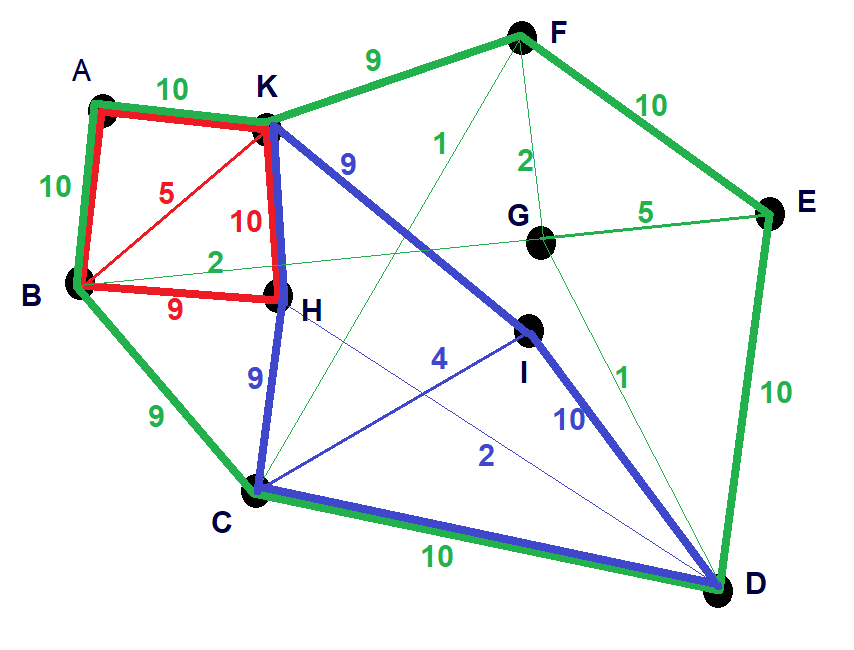
\includegraphics[width=.8\linewidth]{lowwerconnectivity.png}
\caption{An example of lower connectivity regions in the weighted network. Different colors indicate different subnetworks. The center of the network has a cavity and even though the radius of the network is 2 the total flow is slow because of the weak edges. So, communicating via the maximum flow is more efficient than communicating via the shortest paths. For instance, going from node B to E via G is slower than via C and D. Another observation is the difference between the depths of the cavities. The hole surrounded by ABCDEFK is deeper than the hole ABHK because of the strengths of the ambient edges with respect to its inside}
\label{fig:connectivty}
\end{figure}



  In network theory, a k-clique is the subset of nodes in which every node is connected to all k-1 others among the subset. A converse to this concept would be fully disconnected set of nodes which is just a set of nodes with no relations. However, we are assuming our networks has one connected component and nodes are in a relation with the system as a whole. So, a partial converse can be defined as a hole, or a loop, in a network which can be thought of as removing some number of edges from the clique without changing the number of connected components. These regions in terms of brain communication can be characterized by a low connectivity region meaning that information can be carried through the surrounding edges which have relatively high edge weight bypassing the lower connectivity region in the middle, whereas a region without a hole, a full clique, is a stronger connectivity region. If the only concern of the brain was building efficient communication, we would expect it to be a full clique but we would observe neither a modular structure nor the functional variety in this case. Also, we know brain constructs neural pathways in a cost efficient way\cite{costeffic,costeffic1}, whereas constructing a clique is expensive. So, in other words, lower connectivity regions enables networks to optimize the cost and ease of communication.


\begin{figure*}%[tbhp]
\centering
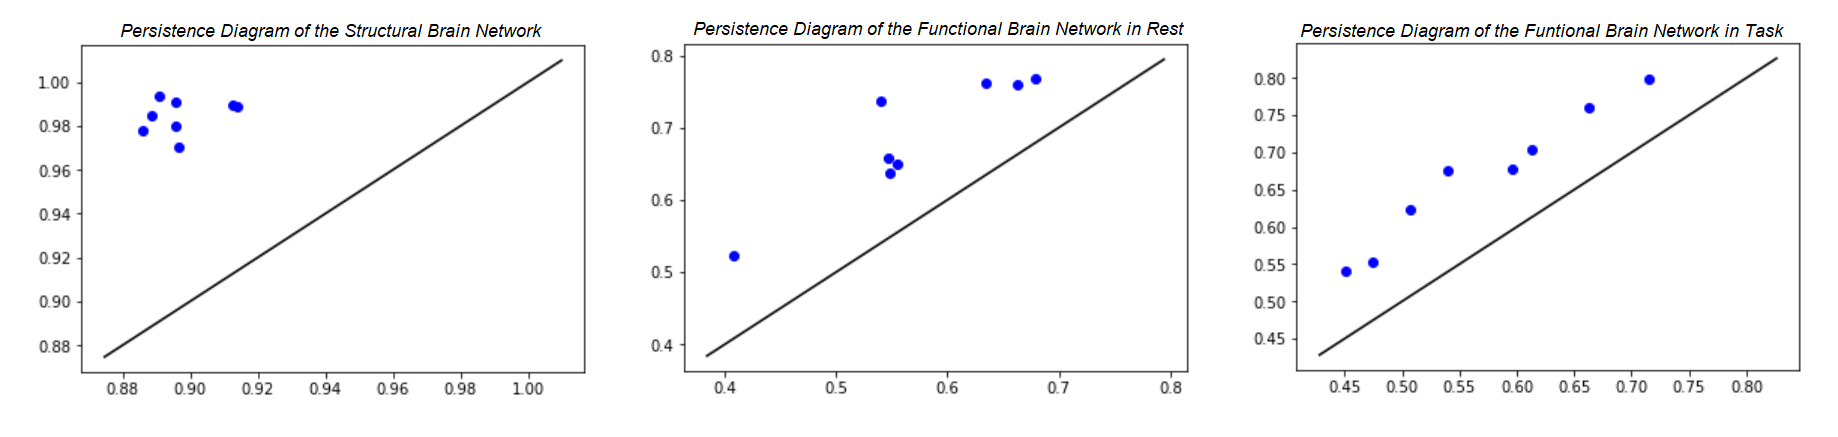
\includegraphics[width=16cm,height=6cm]{peristencediagrams.png}
\caption{Left: Strong edges compounding the loops in the structural brain network comes with strong edges making them a clique, so they don't appear in the persistence diagram. What we see is the weak edges, entering the filtration later on, whose filling edges are absent. Right: loops are appearing at every weight scale; weak edges lack of even weaker edges making them a clique as well as strong edges lacking less strong edges making them a clique. Middle: persistence diagram is more like the one in the task state probably because resting state is the underlying structure of the task.  }
\end{figure*}

On the other hand, a loop in an abstract topological space can be characterized algebraically by the homology groups of that space. Homology is a vector space obtained by quotient of the image of a boundary map by the kernel of the following boundary map such that the composition of the boundary maps is trivial\cite{topologyanddata}. Depending on the dimensions of the boundary maps, the interpretation of homology changes. In the 0-dimensional case, homology counts the connected components of an abstract space. Whereas, in the 1-dimensional case, homology counts loops or 1-dimensional holes and in dimension 2, homology corresponds to the voids enclosed by some volume. It's harder to visualize generic n-dimensional analogues of homology, but rule of thumb is still legit: homology is an algebraic invariant. In the literature, $k$-th Betti number corresponds to the dimension of the $k$-th homology which is what we mean by counting the connected components, loops etc. Given that a network can be constructed via combinatorial structures, so called simplices, every network can be given a topology i.e. every network is a topological object. Therefore, every network is prone to the tools of algebraic topology. So, just like degree, modularity or eigenvalue centrality, homology can be taught of as a network measure whose meaning is slightly less trivial. One of the goals of this paper is, hopefully, fill this gap in the literature.

Persistent homology is a recent technique whose applications gained a lot of attention from different research fields over the past decade. Main idea of persistent homology is that building a nested sequence of subspaces, which is called a filtration, that approximates the original data set. Choosing how to build the filtration from the simplices is like choosing the lenses that one looks at the data set\cite{pershomsimplif}. One can choose different lenses and a maximum dimension $n$ that one wants to approximate the dataset. More formally, let $X$ be the original data set we want to examine and $X_{0}\subset X_{1}\subset...\subset X_{N}$ be the filtration where $X_{N} $ is the $n$-dimensional simplicial complex homotopy equivalent to $X$. Then, one can compute the homology of each individual spaces and keep track of the homological features that persisted in terms of filtration steps.  The main assumption of the persistent homology is that actual signal in the data is going to persist for a long time whereas shorter persistent cycles are likely to be just noise. In the network theory context, a $k$-dimensional homology generator means that somewhere in the complex, $k$-th dimensional subcomplex is missing through all stages of the expansion. This property may be interpreted as the absence in terms of connectivity relations which depend on the lens mentioned above. This approach highlights not only the regions of reduced connectivity but also how network properties evolve along the filtration.

Several applications of persistent homology in the brain network context has been done \cite{dendogram,pershombrainnetw,struc-funcpershom}. Moreover, the idea of homological scaffolds of the brain structure that is used to distinguish the psychedelic state from the resting state  \cite{scaffold} is also one of the constructions we used\cite{strata}. This particular construction enables us to see the communication between the subnetworks, subsystems, of the brain considering the modularity of these systems and assuming the information flow between the submodules are via the links between the hubs and authorities of these submodules.




\section*{Results}

We start with 14 individuals whose structural brain network is obtained via diffusion imaging and functional brain network in resting state is obtained via BOLD signals. For comparison, we also measure the BOLD signals in a modular arithmetic test and turned it into a functional brain network. Then, we averaged the data among 14 individuals and carry on the analysis with only three networks: structural, functional in rest and functional in task. After the computation of 1st homology generators of each networks, we kept the 8 cycles that persisted most in each of them. Figure 3 shows the persistence diagrams corresponding to each instance. The appearance of the lower connectivity regions throughout the filtration is different in each case. Even though we didn't realize a significant difference in terms of persistence durations of these cycles, in the structural network, we noticed all 8 generators born towards the end of the filtration whereas functional brain network in rest shows a little more linear distribution throughout the filtration. Functional brain network in task demonstrates the most linear distribution meaning that the brain turns into a more organized state during a task engaging different levels of lower connectivity regions i.e. several loops born at different weights with pretty much the same depth. On the other hand, in the structural brain network, holes are tend to born and die around the same weight scale. 

Another interesting observation is that in the structural brain network, we observed a lower mesosopic region of connectivity, a loop, between the left and right hemispheres of the brain. Specifically, there exists a hole whose edges run through the brain region LH/SomMotA and RH/SomMotA consistently whereas other loops we found are going through multiple brain regions. This result might be interpreted as, part of the somatomotor system, region A in particular, is structurally a lower connectivity region enabling left and right hemispheres to communicate faster and more efficiently, coordinating multiple bilateral motor tasks.

Then, we compare the results from the homological scaffold networks $N'_{Structural}$, $N'_{Rest}$ and $N'_{MOD}$ in terms of the classical network measures. First thing that draw our attention is that no subcortical region was present in both of the functional homological scaffolds i.e. loops doesn't go through the nodes with ids 200-214 which are precisely the subcortical areas  in the brain. However, there is fair amount of subcortical regions contributing to the structural homological scaffold. Furthermore, another interesting similarity between resting state and task state homological scaffolds is that the most in between edges, the highest edge betweenness centrality, are between the brain regions RH/ContB-RH/DorsAttnA and RH/DorsAttnA-RH/DorsAttnB in both of the functional brain networks-in rest and in task. Then, we further investigated this observation and looked at the degrees of these nodes, shortest paths and compared the betweenness values of these edges. We found out that this part of the network, Dorsal Attention system, is a hub for the functional scaffold incorporating the information all over the brain. Furthermore, we observed betweenness centrality of these two edges are relatively higher in the task state than the resting state.

We kept going investigating these new networks that has constructed in terms of other network measures. We mainly focused on this new structure in terms of information flow and cost efficiency (Table 1) .

\begin{figure*}%[tbhp]
\centering
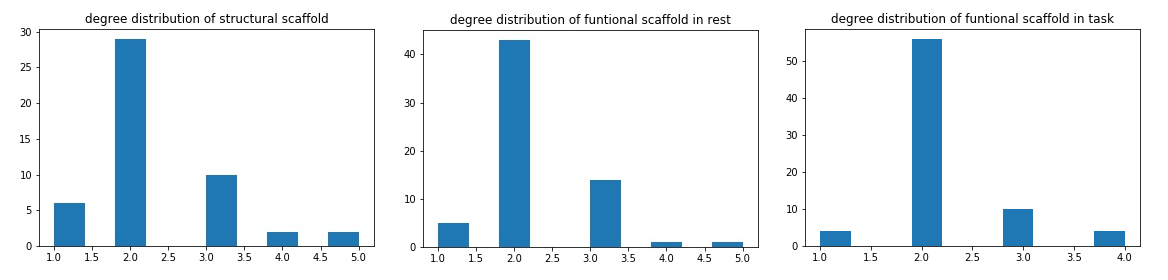
\includegraphics[width=16cm,height=6cm]{degreedists.png}
\caption{Degree distributions of the $N'_{Structural}$, $N'_{Rest}$ and $N'_{MOD}$. Since these networks are consisting of loops i.e. they are union of ring graphs, there shouldn't be any nodes with degree one. However, we know that persistent homology calculation returns the homological information with some noise which are the degree 1 nodes in this case. So, it makes sense that most of the edges have degree two and then degree distribution follows a power law pattern with high clustering and low path length enabling hubs to emerge.}
\end{figure*}

In terms of algebraic connectivity, even though $N'_{Structural}$ and $N'_{Task}$ seemed pretty similar, we couldn't find any reason for this to happen. So, they are not correlated. In terms of transitivity and global efficiency though, $N'_{Rest}$ and $N'_{Task}$ indicated similar behaviour which reinforces the fact that resting state is the underlying structure of the task state. Previous work has also shown that  there is a strong positive association between global efficiency of functional brain networks and intellectual performance\cite{intellectual} just to keep in mind as a future direction.


\begin{table}%[tbhp]
\centering
\caption{Comparison of the algebraic connectivity, transitivity and global efficiency of $N'_{Structural}$, $N'_{Rest}$ and $N'_{Task}$}
\begin{tabular}{lrrr}
Scaffolds & A. Connectivity & Transitivity & Global Efficiency \\
\midrule
1. $N'_{Structural}$ & 0.02353226686 & 0.0769230769 & 0.2331699031 \\
2. $N'_{Rest}$ & 0.09224809273 & 0.1818181818 & 0.4360507246 \\
3. $N'_{Task}$ & 0.02378270622 & 0.1942446043 & 0.4063218390\\
\bottomrule
\end{tabular}

\addtabletext{Comparisons of the network measures based on the information flow}
\end{table}

\section*{Discussion}

In this paper, we tried to understand the effects of lower connectivity regions in the whole brain structure and utilized persistent homology to detect the loops inside of the brain network. We compared structural, functional rest and functional task networks. A lower connectivity region can be thought of as a subnetwork in which the information flow between nodes travels along between the strong edges bypassing the edges with low edge weights. If we would like to use a road network analogy, these lower connectivity regions could be interpreted as travelling through the highways where traffic jams are less likely to occur because of the wide roads, high edge weights in brain network case, is more efficient than travelling through inside of the city where the roads are more narrow and traffic lights are more likely to present. So, even though the total distance travelled is higher on the highways, you can get one point to another quicker compared to driving through inside of the city. There is evidence that many aspects of brain anatomy can be explained in terms of minimising axonal wiring or metabolic running cost\cite{wiringoptim}. Thus, these lower connectivity regions could be one of the mechanisms for efficiently transferring information from one part of the brain to another.

First, we realized that in the structural brain network, the edges with low edge weights are less likely to carry a low connectivity region- no wide roads in the suburbs whereas the loops are more likely to occur between the nodes with strong structural connectivity-highways are built efficiently to travel around downtown. This tells us structural connectivity is constructed in a cost efficient way between the strongly connected brain regions. What this doesn't tell us is that information flow in the low edge weight regions is not efficient simply because loops are not the only mechanisms to built efficiency- a very dense weak edge connections can provide local efficiency still. On the other hand, the functional networks appeared to be cost efficient at every weight scale in terms of this efficiency mechanism i.e. for functional information to flow, brain constructs wider pathways with respect to its surrounding regardless of the weight scale.

Secondly, we observed a specific low connectivity region running between the left and right hemispheres of the brain. We can go ahead and interpret this finding as brain needs structurally large fibers between the left and right hemispheres of the brain compared to its surrounding for somatomotor network to communicate faster and more efficiently, given that somatomotor system is responsible from voluntary muscle movement such as walking which employs both left and right sides of the body simultaneously. This type of bilateralization has shown to be a characteristic of the somatosensory cortex \cite{bilateral}.

The fact that there are no relatively wide pathways going through the functional subcortical areas may tell us that this type of communication is special to cortical regions enabling the distant cortical sites to interact rapidly whereas subcortical regions might not need such type of communication due to its compact nature. This also tells us how the structure and function might influence each other. Physically far brain sites are in need of relatively wider pathways, this special type of construction in particular, which are mostly present in the upper cortex. In fact, ranking of brain regions according to their score on multiple centrality metrics (e.g., degree, betweenness, and closeness centrality) confirmed a central network position for the medial parietal, frontal and insular regions\cite{structure-funct} and findings shown to be consistent across different cortical and subcortical parcellations. Network analysis now suggests
that the integrative and diverse properties of these regions
are due to their central embedding within the connection
topology of the brain, which is in line with the idea that
functional properties of regions are shaped by their connectional fingerprint.

\begin{figure*}%[tbhp]
\centering
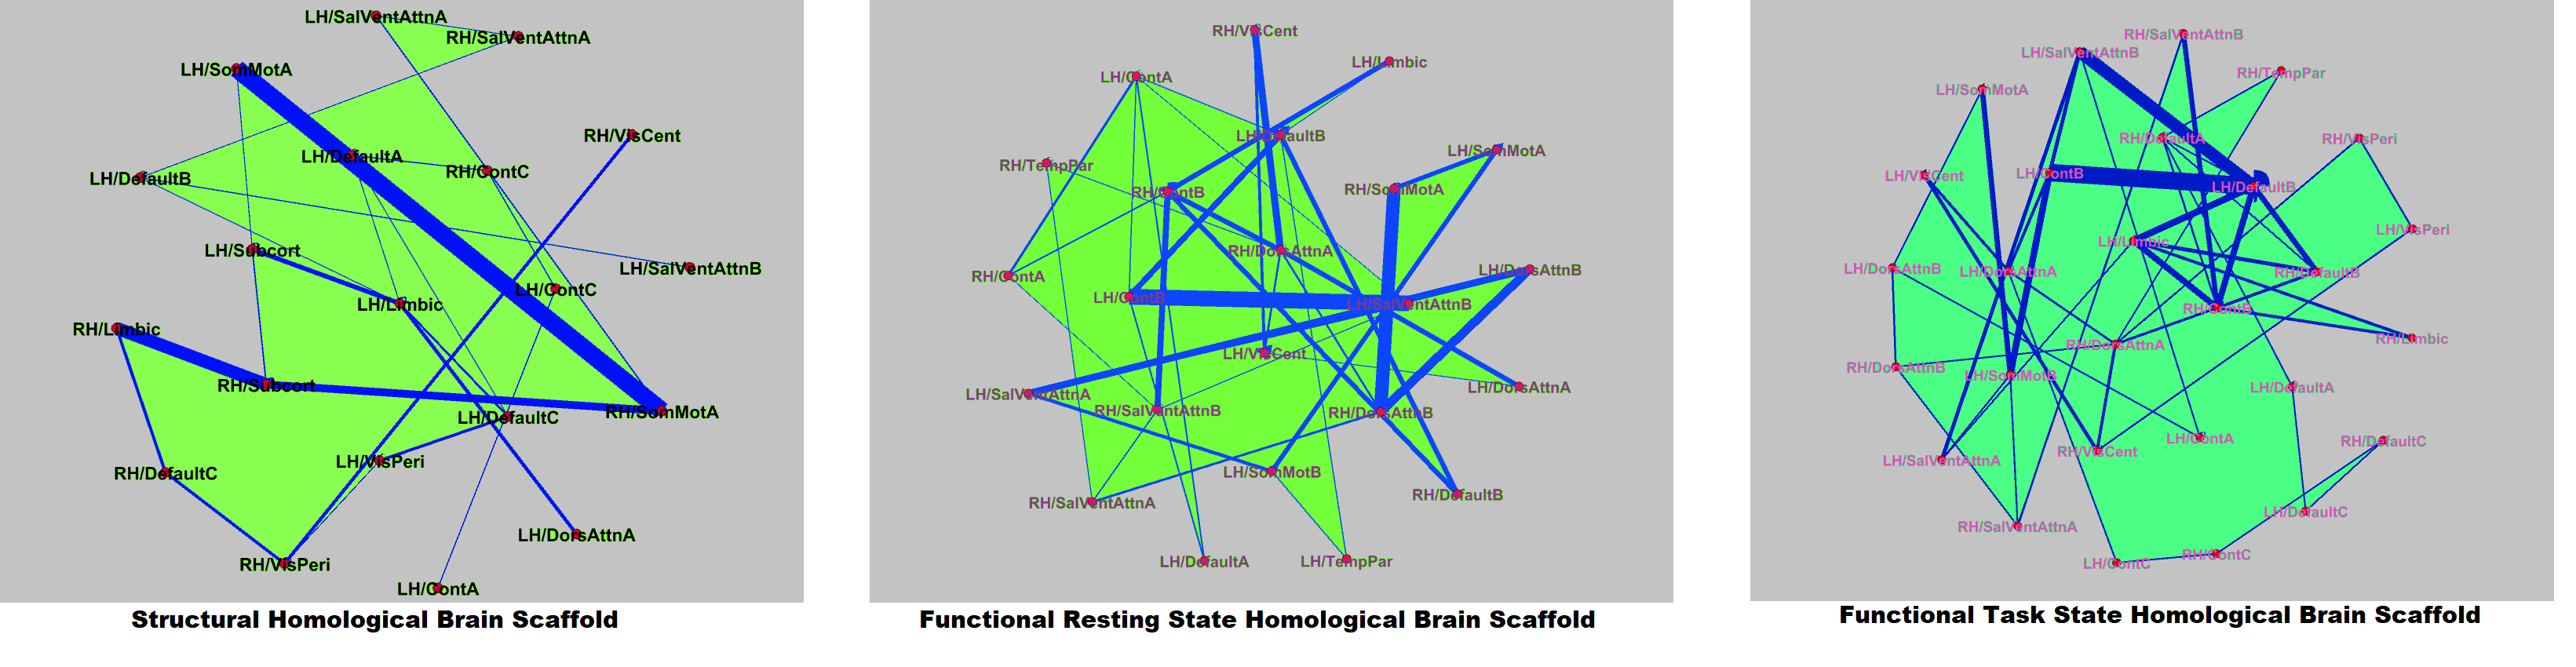
\includegraphics[width=18cm,height=6cm]{strucscaf.png}
\caption{Visualization of the persistence scaffolds that we constructed. Left: $N'_{Structural}$. Middle: $N'_{Rest}$. Right: $N'_{Task}$  }
\end{figure*}


The homological scaffold information provided us being able to extract these edges with relatively high weights and aggregate them on a new network by assigning a new edge weight depending on the importance of the edge during the filtration process(Figure 5). A large total weight, persistence, for a link in the persistence scaffold implies that the local structure around that link is very weak when compared to the weight of the link, highlighting the link as a locally strong bridge. 
We want to highlight the fact that the homology generators contains some topological noise which can be seen from the degree distribution of these networks-occurrence of degree one nodes (Figure 4). However, we can correct this issue by just neglecting these nodes and their connecting edges. A more detailed and technical handling of this issue can be found \cite{optimalc1,optimalc2} so that we have a nice and clean topological summary. 

The most striking information we stumbled upon in the scaffolds is the coincidence of the two of the most in between edges in both of the functional brain networks. Moreover, the nodes these most in between edges connect are corresponding to the highly connected nodes or hubs of the functional scaffolds. When we investigate further these subnetworks, Dorsal Attention and Control, these systems with low path length and high clustering are mediating interactions between various sensory and motor systems in the macaque cortex \cite{smallworld1,smallworld3}. Also, considering that our task was a modular arithmetic test, our findings reinforces that Dorsal Attention is not only a functional hub but also a central junction for cognitive information flow.



\section*{Methods and Materials}

\subsection{Structural and Functional Correlation Dataset} Structural connectivity from 14 individuals obtained via diffusion spectrum imaging(DSI) data and tractography. As a result, 17 systems in each hemisphere further divided into 107 cortical and subcortical regions of interests, making 214 nodes in total.
The empirical resting-state functional connectivity was also obtained from the same 14 subjects by measuring the corresponding fMRI BOLD signals and divided into 214 brain regions for a legit comparison between function and structure. For the task performance, we chose a modular arithmetic test and acquired the functional connectivity matrices in task ($214\times 214$) for every individual again via the correlation between nodal activities on the basis of blood oxygenation level-dependent functional MRI. 

For our analysis, we mainly used the matrices which are averaged along the individuals and carry on the analysis via three networks; structural, functional resting-state and functional task.



\subsection{Persistent Homology as a Lower Connectivity Region Measure}
As we mentioned earlier, brain networks have small world properties. It is shown that persistent homology of random networks generated by different mechanisms such as Erdos-Renyi, preferential attachment and exponential degree distribution have characteristic topological summaries even for different parameter selections \cite{pershomcompnetw}.



We started by indexing the filtration $X_{0}\subset X_{1}\subset ...\subset X_{n}=X$ by the ranked edge weights in descending order. This will provide the edges with higher weight entering the filtration earlier and edges with lower edge weight later enabling the cavities in the network to be more significant before they get filled(or reinforced) by a 2-cell, or a 3-clique which is nothing but a triangle. We used a clique complex of dimension 2 to only observe loops, namely, our construction goes as follows: given that we have a weighted undirected network $N=(V,E,\omega)$, all 0-cells, the set of vertices $V$, are assumed to be having weight $0$, so they are going to be present in the space $X_{0}$. Then, in the first filtration step $X_{1}$, edges with maximum weight $\omega_{max}$ are going to enter the filtration. Then, in $X_{2}$, some edges with weight $\omega<\omega_{max}$ are entering the filtration in order to have $X_{1}\subset X_{2}$ and so on. Finally, the weight of a 2-cell is determined by minimum of it's coboundary so that at each step we'll have a closed 2-skeleton. Persistent homology computation can be reduced to gaussian elimination and can be done by the algorithm given in the original paper\cite{zomorodian} easily. Although, there are several packages in Python and MatLab that computes the persistent homology of a filtration, a very good review article can be found \cite{roadmap}, we prefer to use our own(eztda) due to time limitations.

After computing the homology generators, we use a persistence diagram or a barcode \cite{barcode} which refer to the topological summaries of the data. A persistence diagram is a scatter of points above the $x=y$ line that demonstrates the birth and death times of the homology generators in a compact fashion. The birth time $\beta_{c}$ represents the filtration index in which that homological feature has appeared and the death time $\gamma_{c}$ represents the filtration index in which the homological feature disappear giving us a total survival time $\pi_{c}=\gamma_{c}-\beta_{c}$ which we call persistence.  The further up a point is from the diagonal, the more meaningful the information that point represents.

\subsection{Homological Scaffolds of the Reduced Connectivity Regions}
After computing the homology generators for the three main networks, we apply a persistence threshold keeping the most persistent 8 cycles in each network. A cycle $g_{c}$ is a chain of edges enclosing a loop in the network. So, to see that which brain regions are contributing to the reduced connectivity of the brain systemwise, we grouped together the 214 nodes in the networks according to the systems and hemispheres that they belong to and added the homology generators as edges with weight summed persistence value. More formally, let $N=(V,E,\omega)$ be as before, we constructed a new network $N'=(V',E',\omega^{\pi})$ from the homological information such that $V'=\{v_{i_{k}}|,i=1,..,34, k $ is the number of nodes in each system \} and $E'=\bigcup_{c\in C}g_{c}$ where $C$ is the set of 8 cycles found by the persistent homology computation and the weights are given by:

\begin{align*}
\omega^{\pi}_{e'}=\sum_{g_{c}|e'\in g_{c}}\pi_{g_{c}} \numberthis\\
\end{align*}

We continued our analysis with these three new networks $N'_{structural}, N'_{rest}$ and $N'_{task}$.





\acknow{Johan Nakuci provided the structural/funtional connectivity dataset and Sarah Muldoon provided the eztda Python package for the homology computation.}

\showacknow{} % Display the acknowledgments section

% Bibliography
\bibliography{pnas-sample}

\end{document}